
\label{chapter:fund_teo}
Este capítulo tem como objetivo apresentar os conceitos e definições abordados neste trabalho, tais como: Sistemas Embarcados, Modelos Formais para Verificação de Sistemas, Visão Computacional e Reconhecimento de Padrões.
  
    
    
\section{Sistemas Embarcados} 

Sistemas computacionais estão por toda parte e muitos deles estão em computadores pessoais, já sistemas embarcados são um tipo específico de sistema computacional que pode ser encontrado em uma grande gama de dispositivos, desde \textit{notebooks, tablets} a jogos eletrônicos portáteis, máquinas de fax, entre outras coisas como eletrodomésticos~\cite{vahid:2002}.

Segundo~\citeonline{vahid:2002}, um sistema embarcado é qualquer sistema computacional que não seja um computador pessoal ou \textit{workstation}. \citeonline{heath:2002} define sistemas embarcados como sistemas baseados em microprocessadores ou microcontroladores (ver Seção~\ref{Sect:Micros}), construídos para executar uma \textbf{função específica} ou grupos de funções programadas. Os sistemas embarcados não são projetados para serem reprogramados da mesma forma que computadores pessoais.
% 
Um dos exemplos citados por \cite{heath:2002} como sistema embarcado é uma máquina de lavar, que possui vários ciclos de lavagem, painéis para acompanhar os ciclos e controle dos motores, e bombas de água.


Já \citeonline{schlett:1998} diz que um sistema embarcado precisa executar uma tarefa específica com o menor custo energético e monetário possível.
%O custo energético é um dos grandes desafios encontrados no desenvolvimento de sistemas embarcados.
Neste sentido, segundo \citeonline{vahid:2002}, algumas características de sistemas embarcados são:\begin{itemize}
\item Função única: Sistemas que são programados para um tarefa específica, que pode se repetir várias vezes.
\item Fortemente limitado: Sistema com limitações definidas nas suas métricas de projeto, como de desempenho, consumo de energia, preço e dimensões.
\end{itemize}

Mesmo com a necessidade de desenvolvimento de \textit{chips} mais rápidos e mais baratos, a necessidade de adicionar ou remover funcionalidades de um projeto de sistema embarcados também é muito importante. Encapsulando partes do sistema ao \textit{software} é possível fazer atualizações no sistema sem a necessidade de mudar o \textit{hardware}, isso diminui os custos de fabricação, fazendo com que vários sistemas embarcados utilizem o mesmo \textit{hardware} \cite{heath:2002}. Esses artifícios são vantagens que fazem com que muitos dos produtos utilizados pela população (como micro-ondas e alguns eletrodomésticos) se tornem mais baratos.


% =========================================================
\subsection{Microcontroladores x Microprocessadores}
\label{Sect:Micros}
% =========================================================        


Segundo \citeonline{heath:2002}, os computadores modernos (como \textit{desktops} e \textit{laptops}) são baseados em microprocessadores, permitindo-os realizar várias funções, enquanto outros sistemas baseados em microcontroladores, são limitados a apenas um ciclo repetido da mesma tarefa. Os microprocessadores foram originalmente desenvolvidos para substituir as primeiras calculadoras, com chips que de alguma forma pudessem ser reprogramáveis, que ao invés de desenvolver outro chip só mudasse apenas o código.

Ainda por \citeonline{heath:2002}, O termo design de sistemas embarcados abrange uma enorme gama de projetos de microprocessadores, não sendo exclusivamente para um microcontrolador simples, podendo ser um computador pessoal que executa certos \textit{softwares}.\par Microcontroladores são compostos por vários componentes integrados a ele, como RAM, interface de entrada e saída e uma memória re-programável~\cite{white:2011}.

%Segundo \citeonline{white:2011} define microcontroladores como processadores com componentes atrelados a ele, com memória re-programável

Sistemas embarcados derivaram de processadores desenvolvidos para o mercado de computadores domésticos, com algumas diferenças no consumo energético, preço e componentes atrelados à CPU. Outras diferenças são o tempo de resposta de interrupções, a quantidade de memória e portas paralelas \cite{schlett:1998}.

Um exemplo de um sistema baseado em microcontrolador é o \textit{Arduino Uno} \cite{Arduino2018ArduinoRev3} que é uma microcontrolador que possui $14$ pinos digitais, $6$ portas analógicas, cristal de quartzo com frequência de $16$Mhz, conexão USB e entrada de alimentação eletrica. O \textit{Arduino} pode ser reescrito várias vezes utilizando um computador e no pior dos casos você pode substituir o microcontrolador com um preço acessível \cite{Arduino2018ArduinoRev3}.


Existem também os \textit{Single Board Computers}, um bom exemplo é o \textit{Raspberry PI}, que segundo \citeonline{RaspberryPi2016DATASHEETCM3L}, possuem processador e memória integrados, os caracterizando como microcontroladores ou modulo computacional. As vantagens da utilização são por seu baixo custo, baixo consumo energético e alta rentabilidade e grande quantidade de portas para uso geral como pode ser visto no \textit{datasheet} da \autoref{fig:raspsheet}. 


 \begin{figure}[H]
	\centering
    	\caption{\label{fig:raspsheet} CM3/CM3L Diagrama }
		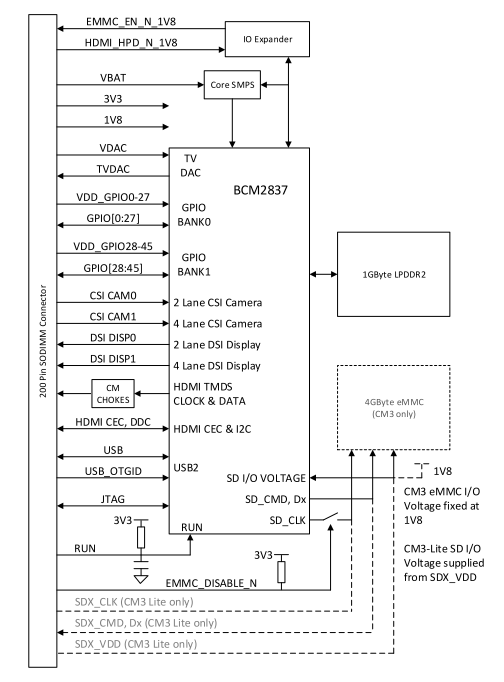
\includegraphics[width = 0.8\textwidth]	{resources/raspsheet}
    	\legend{Fonte:\citeonline{RaspberryPi2016DATASHEETCM3L} }
\end{figure}

\label{jain:raspberry}
Um bom exemplo de um sistema construído utilizando um \textit{Single Board Computer}, é o sistema proposto por \citeonline{jain2014raspberry}, que utiliza Raspberry Pi para automação residencial através da internet utilizando e-mail. 


% =========================================================
\subsection{Internet das Coisas(IoT - Internet of Things)}
% =========================================================

A Internet das Coisas (IoT - \textit{Internet of Things}) é paradigma que está ganhando espaço no cenário moderno de telecomunicações sem fio. Sendo seu conceito básico conectar uma vasta quantidade de coisas ou objetos (casas, carros, sinais de trânsito e outros), fazendo-os interagir entre si para alcançar um objetivo em comum \cite{atzori2010internet}.


Segundo \cite{xia:2012} a Internet das Coisas é um conceito que interligará todos os dispositivos através de sistemas embarcados, formando uma rede de dados inteligente, ubíqua e distribuída. Os dispositivos podem trazer avanços que irão melhorar a qualidade de vida, facilitando a comunicação entre pessoas e dispositivos.

Todos os dispositivos ao nosso redor estarão conectados a internet, isso resultará numa enorme quantidade de dados que terão de ser processados e apresentados sem falhas de forma eficiente. A computação em nuvem pode oferecer uma infraestrutura de ponta a ponta, entre o dispositivo e o servidor satisfazendo essa demanda de qualquer lugar \cite{Gubbi:2013}.

Internet das Coisas é sobre ampliar o escopo de conexões para objetos que não são convencionais de estarem conectados à rede. Por esse motivo uma grande quantidade de soluções de comunicação foram introduzidas, visando o melhor custo energético \cite{siekkinen2012low}. 
% E a utilização dessa visão neste trabalho será onde 

Na tentativa da caracterização da Internet das Coisas, A \autoref{fig:iotoverview} coloca os principais conceitos, tecnologias e padrões na visão desse paradigma, destacando e classificando as diferentes visões que resultam na Internet das Coisas, mostrando o melhor resultado de uma convergência.

 \begin{figure}[H]
	\centering
    	\caption{\label{fig:iotoverview} Paradigma "Internet das Coisas" (IoT) como resultado da convergência de diferentes visões }
		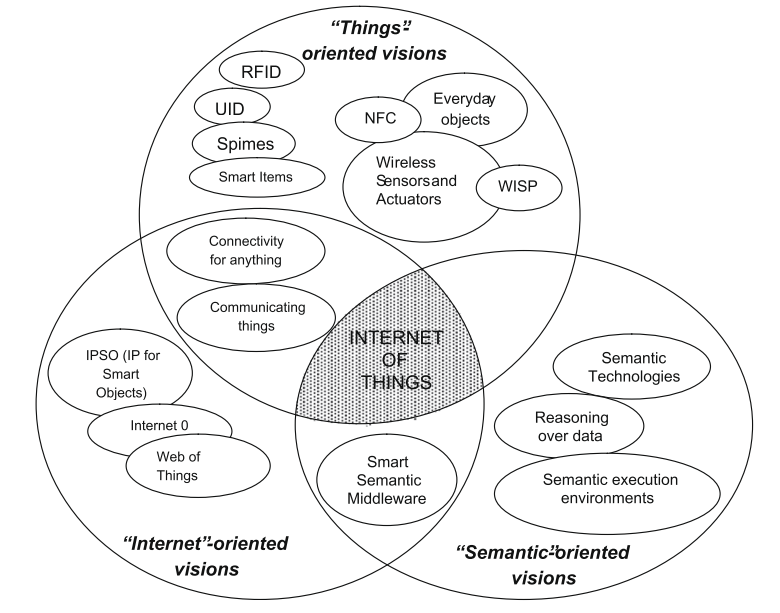
\includegraphics[width = 0.8\textwidth]	{resources/iotoverview}
    	\legend{Fonte: \cite{atzori2010internet}}
\end{figure}

O sistema proposto por \citeonline{jain2014raspberry}, mostra uma placa de sistema integrado, que possibilita automação residencial através da utilização de e-mails. O sistema funciona inicializando o ambiente e logando o e-mail do usuário, em seguida ele lê os assuntos dos e-mails, comparados com os comandos armazenados anteriormente em um banco de dados. Esses comandos são usados para controlar os dispositivos da casa. Segundo \citeonline{jain2014raspberry}, o \textit{Raspberry Pi} foi escolhido como unidade de processamento por seus benefícios e custos econômicos. 

A \autoref{fig:jainraspberr} ilustra como a configuração do sistema proposto, sua conexão e controle dos relês que controlam os dispositivos interligados. 

 \begin{figure}[H]
	\centering
    	\caption{\label{fig:jainraspberr} Visão do sistema proposto por \citeonline{jain2014raspberry} }
		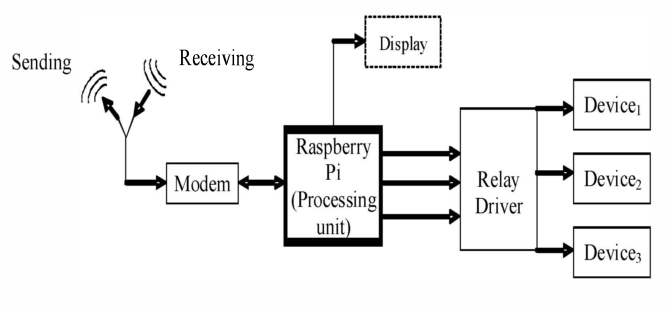
\includegraphics[width = 1\textwidth]	{resources/jainraspberry}
    	\legend{Fonte: \cite{jain2014raspberry}}
\end{figure}


% =========================================================
\subsection{Baixo consumo de energia}
% =========================================================

Os dispositivos que compõem a Internet das Coisas são caracterizadas por utilizar poucos recursos, em termos de computação e capacidade energética. Isso requer certa atenção, já que novos projetos terão que levar em consideração à eficiência dos recursos e problemas de escalabilidade \cite{atzori2010internet}.

Com o avanço da Internet das Coisas, uma grande demanda de dados surgiu e por sua vez a alocação e gerenciamento de dados se tornaram um problema crítico. Atualmente a internet utiliza 5\% da energia gerada com a solução desses tipos de problemas, e tende a crescer cada vez mais~\cite{Gubbi:2013}.



%Geralmente há restrições no \textit{hardware} e \textit{software}\todo{Apresentar exemplos}. As restrições de \textit{hardware} ajudam a limitar a utilização de recursos energéticos e monetários, e as de \textit{software} limitam o programa a um determinado ciclo, podendo esse ser determinístico ou/e tempo real, reagindo de forma rápida e tolerante a falhas. Essas restrições são dadas pois um sistema embarcado faz parte de um sistema maior, muito mais composto. %informações do slide irei citar 19/01/18

Um sistema embarcado é projetado para executar tarefas específicas, limitando alguns recursos como memória RAM, armazenamento, periféricos e ciclos de processamento e velocidade de processamento. Um exemplo prático é adicionar mais linhas de códigos, usando mais armazenamento, melhorando o tempo de execução do código, outro exemplo é reduzir a velocidade de processamento para reduzir o consumo energético \cite{white:2011}.

De acordo \citeonline{Marwedel:2010}, que descreve uma série de requisitos e abordagens para especificar um dado sistemas embarcados, essas especificações geram modelos do sistema em desenvolvimento. Esses modelos são descritos em linguagens, essas linguagens devem ser capaz de representar alguns características, bem como:
\begin{itemize}
    \item \textbf{Sincronização e Comunicação}: onde os componentes devem se comunicar e estarem sincronizados. sem comunicação não há cooperação entre eles.
    
    \item \textbf{Comportamento Temporal}: levando em consideração há existência de muitos sistemas embarcados em tempo real. Sendo uma das características mais importantes de alguns sistemas embarcados. Na ciência da computação o tempo é dado de maneira abstrata, a notação $O$ é um desses exemplos, que reflete o grau de crescimento de uma função, usado frequentemente para medir o tempo de execução de algoritmos, mas falha ao descrever a execução real de tempo.
    Para sistemas em tempo real, é necessário quantificar o tempo. Para isso algumas técnicas podem ser utilizadas, como: \textbf{medir o tempo utilizado}, meios de \textbf{atrasar um processo} por determinado período de tempo, \textbf{especificar \textit{timeouts}}.  
    
    \item \textbf{Propriedades não-funcionais}: Sistemas embarcados em desenvolvimento devem possuir um número de propriedades não-funcionais, como tolerância a falha, tamanho, extensibilidade, perspectiva de vida, consumo energético, peso e outros.
\end{itemize}

\citeonline{Marwedel:2010} ainda afirma que melhorar as tecnologias de baterias, nos ajudará a conseguir uma melhor duração para baterias, mas a limitação térmica nos impede de utilizar essa energia por muito tempo, devido a problemas de superaquecimento do dispositivo. Devido a esses problemas de temperatura, dispositivos estão sendo projetado com sensores para detectar quando há superaquecimento, regulando o dispositivo para o evitar que isso aconteça. 


% =========================================================
\section{Modelos formais para verificação de sistemas}
% =========================================================
%falar sobre verificação de sistemas. A importância e onde é usada. Falar sobre modelos formais. Falando que a seção fala sobre exemplos de modelos formais. 
 
De acordo com \citeonline{Baier:2008} sistemas de Tecnologia da Informação e Comunicação (TIC) estão crescendo rapidamente, e seu funcionamento de forma eficaz é fundamental. Esses sistemas estão se tornando cada vez mais complexos e estão ganhando espaço no cotidiano através da internet e de todos os tipos de sistemas embarcados. Sistemas TIC estão por toda parte, eles controlam a maioria dos dispositivos de uso cotidiano (como por exemplo um sistema para controle da casa, como o sistema proposto por \citeonline{jain2014raspberry}).

A dependência do uso de sistemas embarcados tornam sua eficácia fundamental para sociedade. Esses sistemas oferecem um bom desempenho em tempo de resposta e capacidade de processamento. O mal funcionamento desses sistemas podem ameaçar nossas vidas, e podem ter consequências financeiras substanciais para o fabricante. Sistemas TIC eficazes são fundamentais para a sobrevivência de uma empresa \cite{Baier:2008}.

Um exemplo clássico de uma falha catastrófica, é a falha do lançamento do Ariane 5. Em 4 de Junho de 1996, o lançamento do foguete Ariane 5 terminou com uma falha catastrófica, com apenas 40 segundos após o início da sequência de lançamento. As condições de lançamentos eram ideais, nenhum problema climático ou pertubações no campo magnético. O problema no lançamento foi o \textbf{sistema de controle de voo}, mais precisamente no \textbf{sistemas de referência inercial}, causando uma série de reações em cadeia até a auto-destruição do foguete \cite{lions1996ariane}.

Após testes posteriores foi comprovado que o causa técnica foi um erro de operando no momento de conversão do variável do viés horizontal, fazendo o sistema de referência inercial sobrecarregar e parar. foi comprovado que nem todas as operações estavam protegidas após uma análise em todos os códigos que demonstravam risco \cite{lions1996ariane}. 


O crescimento na complexidade dos sistemas TIC mostram que eles não estão mais isolados, agora podem fazem parte de um grande sistema, conectando e interagindo com vários outros outros componentes, tornando esses sistemas vulneráveis a erros. 
A concorrência e o não determinismo que são fundamentais para a modelagem dos sistemas integrados, tornando a utilização de técnicas padrões muito difícil \cite{Baier:2008}.

Técnicas de verificação são aplicadas a sistemas TIC de forma mais confiável. A verificação de sistemas trabalha pra estabelecer que o produto possua certas propriedades, como certificar que o sistema não entre em uma situação de \textit{deadlock}. A falha é encontrada quando o sistema não cumpre todas as propriedades especificadas \cite{Baier:2008}.


%\subsection{Máquina finita de Estados}
%yMáquina finita de estados é um automato que ajuda a demonstrar o fluxo de um sistema computacional. (pré-texto) 

% =========================================================
\subsection{UML}
% =========================================================

Segundo \citeonline{rumbaugh2017unified} UML (\textit{Unified Modeling Language)} é uma linguagem de modelagem visual que tem como intuito de utilizar todos os métodos de desenvolvimento de software, extraindo melhor para especificar, visualizar, desenvolver e documentar os artefatos de um sistema em nível de software, capturando estáticas informais e dinâmicas do comportamento de um sistema. Alguns diagramas da UML de acordo com \citeonline{rumbaugh2017unified} são:

\begin{description}
    \item[Diagrama de Classe:]Os principais componentes do diagrama de classe são classes e suas relações, associação e generalização, mostrando algumas dependências e utilização de cada elemento.
        
    \item[Diagrama de Caso de Uso:]Os principais componentes do diagrama de Caso de Uso são os atores e as funcionalidades. O diagrama modela o sistema, expressando a relação dos atores com o sistema em si.
 
    
    \item[Diagrama de Sequência:]O diagrama de sequência, que será utilizado nesse trabalho para validar algumas ações. Como ilustra a \autoref{fig:sequencerumbaugh}, o diagrama de sequência possui um grupo de mensagens que estão organizados em uma sequência de tempo, toda classe é definida como uma linha do tempo, no exemplo da \autoref{fig:sequencerumbaugh}, os objetos ativos são linha temporais exibidas pelas linhas verticais, mostrando os processos que são relacionados com elas durante seu tempo de vida. As mensagem são representadas por setas entre as linhas de tempo.
    
        \begin{figure}[H]
    	    \centering
        	\caption{\label{fig:sequencerumbaugh} Diagrama de sequência }
    		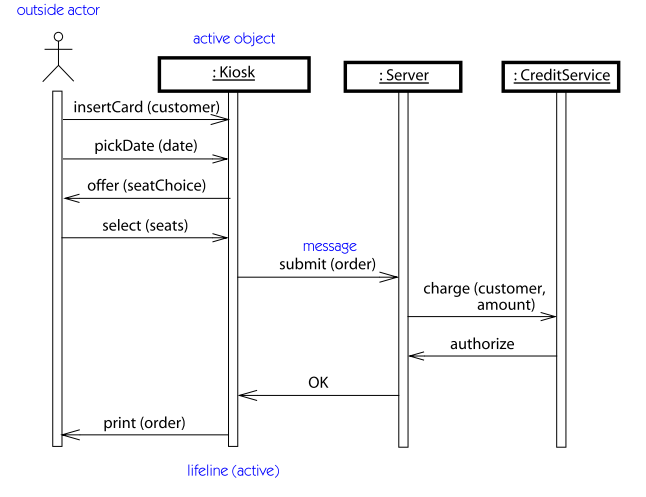
\includegraphics[width = 0.8\textwidth]	{diagramas/sequencediagramrumbaugh}
        	\legend{Fonte: \cite{rumbaugh2017unified}}
        \end{figure}


    
    \item[Diagrama de Colaboração:]O diagramas de colaboração modelam os objetos e links que são significativos dentro de uma interação. O papel das classes descreve o que acontece com um objeto e o papel do associador descreve a relação com a colaboração dos objetos.

    
    \item[Diagrama de Estados:]A máquina de estados modela as possibilidades de um objeto de uma classe. os principais componentes são os estados e as transições. Cada estado modela uma linha temporal dado determinada condição, condição essa que pode levar o objeto a um novo estado.

      
    
    \item[Diagrama de componentes:]Os diagramas de componentes modelam os componentes a serem utilizados na implementação de um sistema, definindo dependências entre os componentes, a nível \textit{software}, podendo avaliar o impacto de uma possível mudança nos componentes.

    
\end{description}



A utilização de UML nesse trabalho se dará pela utilização de diagramas de sequência que mostrarão como o fluxo do software irã ocorrer. De acordo com \citeonline{rumbaugh2017unified}, diagramas de sequência mostram a iteração em uma forma bidimensional, onde o eixo vertical é o tempo de vida do processo e o eixo horizontal mostra as regras de transição como pode ser visto na Figura~\ref{fig:sequencerumbaugh}. %Essas regras são definidas pelas setas que são os processos do software.

Já \citeonline{Cunha2011FormalContext} diz que nos diagramas de sequência as ações são organizadas por tempo, mas não exploram as relação dos objetos. Os diagramas de sequência mostram todo o processo de trocas de mensagens dos objetos, mapeando todo o ambiente mostrando como os objetos colaboram entre si para obter sucesso. Um exemplo é a \autoref{fig:sequencerumbaugh}, que mostra um diagrama de sequencia, com ator, processos e ações que são executas em certa ordem. 



%falar o que é. pra que é usado, e onde será usado no trabalho

% \todo{Computer vision is a vast fi eld. Th is book will give you a basic grounding in the fi eld, but we also recom- mend texts by Trucco [Trucco98] for a simple introduction, Forsyth [Forsyth03] as a comprehensive refer- ence, and Hartley [Hartley06] and Faugeras [Faugeras93] for how 3D vision really works}
% wa

\subsection{Redes de Petri}

Redes de Petri são modelos gráficos e matemáticos que podem ser aplicados em diversos sistemas, como parte da validação . Um método capaz de descrever e analisar as transições do sistema, podendo ele ser concorrente, assíncrono, distribuído, paralelo e não-determinístico. O modelo gráfico é capaz de auxiliar na visualização do fluxo, e a ferramenta matemática pode estruturar equações matemáticas para validação de propriedades formais do sistema analisado. O comportamento de sistemas pode ser descrito em estados, um estado em uma rede de Petri é alterado de acordo com a regra de transição~\cite{murata:1989}.

Já \citeonline{peterson:1981} diz que a aplicação das redes de Petri são através de modelagem. Um modelo é uma representação, muitas vezes em termos matemáticos, descrevendo quais são os atributos importantes do sistema estudado. Manipulando a representação do sistema pode facilitar o levantamento de informações sem prejudicar o projeto real, prevendo algum empecilho que possa ocorrer.  

A estrutura de uma rede de Petri graficamente estruturada como um grafo direcionado, que consiste em estados e transições, tendo dois tipos de nós, círculos que representam estados, e barras que representam transições que se conectam com setas aos estados e vice-e-versa, indicando entrada e saída. Redes de Petri são multígrafos bipartidos, uma vez que permitem múltiplas setas partindo de um único nó do grafo até outro, podendo essas setas serem particionadas em dois grupos (estados e transições) e (transições e estados), uma vez que essas setas sejam direcionado a um elemento de outro grupo \cite{peterson:1981}. 

De acordo com \citeonline{murata:1989}. a definição formal de uma rede de Petri é dada por:
uma rede quíntupla  \(PN = (P, T, F, W, M_0)\), onde:

\begin{description}
    \centering
    \item[] \(\textbf{P} = \{p_1, p_2, \ldots , p_m\}\) é um conjunto finito de lugares,
    \item[] \(\textbf{T} = \{t_1, t_2, \ldots, t_n\}\) é um conjunto finito de transições,
    \item[] \(\textbf{F} \subseteq (P \times T) \cup (T \times P)\) é um conjunto de arcos (relação de fluxo),
    \item[] \(\textbf{W}: \textbf{F} \to \{1,2,3,\ldots\}\) é uma função de peso,
    \item[] \(\textbf{M}_0: \textbf{P} \to \{0,1,2,3,\ldots\}\) é a marcação inicial,
    \item[] \(\textbf{P} \cap \textbf{T} = \emptyset\) e \(P \cup T \neq \emptyset\)

\end{description}
   

Segundo \citeonline{rumbaugh2017unified}, ainda que uma máquina de estados seja bem estruturada, um grupo de transições pode levar a sérias inconsistências, incluindo \textit{deadlocks} e outros problemas. Esses problemas foram bastante estudados na teoria das redes de Petri. 

 \begin{figure}[H]
	\centering
    	\caption{\label{fig:petri}Regra de transição}
		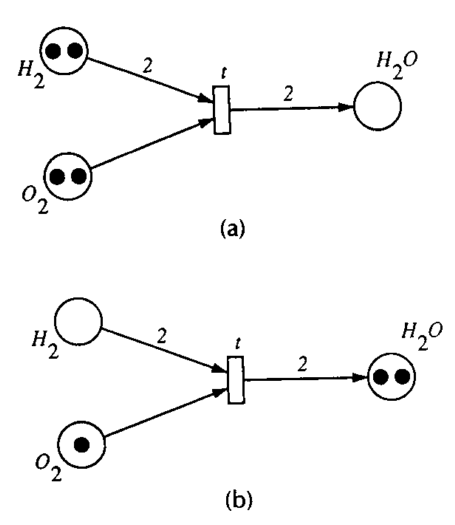
\includegraphics[width = 0.3\textwidth]	{resources/petri}
    	\legend{Regra de transição, (a) aceitação antes da transição \textbf{\textit{t}}. (b) iteração após aceitação de \textbf{\textit{t}}, \textbf{\textit{t}} está desativado.\cite{murata:1989}}
\end{figure}


\section{Visão Computacional}

A visão humana não tem dificuldades em identificar pequenas variações na translucidez e sombreamento em imagens, distinguindo os objetos da imagem que é fundo. Temos certa facilidade em identificar estruturas tridimensionais, podemos diferenciar formatos, texturas, cores e pessoas em imagens, e até mesmo dizer que sentimentos eles podem estar sentindo, apenas olhando fotos \cite{szeliski2010computer}.
% 
A visão computacional é uma forma de emular a visão humana, possuindo imagens como entrada, e sua saída é a interpretação dessa imagem \cite{marengoni:2009}.

\citeonline{bradski:2008} definem uma parte da vasta área da visão computacional como uma transformação de dados de uma imagem em uma nova representação para atingir um objetivo específico, como deixar a imagem em escala de cinza. Essas transformações precisam de contexto, como especificar distância, referências de onde a imagem foi tirada, ou o que pode conter na imagem.

De acordo com \citeonline{marengoni:2009}, a necessidade de uma etapa de pré-processamento é importante quando queremos extrair informações. Essa etapa de pré-processamento envolve o processamento de imagens, que muitas vezes precisam ser convertidas para certo formato ou tamanho com a necessidade de serem filtradas para remoção de ruídos provenientes dos processos de aquisição de imagem, como por exemplo o tipo de sensor utilizando na hora da captura ou até mesmo a iluminação do ambiente assim como condições climáticas.

Os filtros são ferramentas básicas que podem remover ruídos de imagens, filtros podem ser espaciais, atuando diretamente na imagem, ou filtros de frequência, necessitando de uma transformação no seu domínio, geralmente essas transformações de domínio são feitas utilizando das transformadas de Fourier, para assim então serem aplicados os filtros e em seguida transformadas novamente para o domínio espacial \cite{marengoni:2009}.

De acordo com \citeonline{gonzalez1992digital}, existem três níveis de processamento de imagens, baixo nível, nível médio, e alto nível. O processamento em baixo nível envolve operações primitivas como processamento para redução de ruídos, aprimoramentos de contraste e aprimoramentos de nitidez. Esse nível é caracterizado por receber como entrada uma imagem e retornar uma imagem como saída. Processamento em nível médio em imagem envolvem tarefas como segmentação que particionam a imagem em regiões, classificando objetos. Esse nível é caracterizado por receber imagens como entrada e retornar atributos extraídos das imagens de entrada, como contornos. O processamento de imagem em alto nível envolve a compreensão do computador na hora do reconhecimento de objetos, realizando funções cognitivas normalmente associadas a visão.

Alguns exemplos de níveis:

\begin{itemize}
\item Baixo-nível: 
	Pode ser associado a operações como redução de ruídos ou níveis de contraste da imagem \cite{marengoni:2009}. Um exemplo pode ser visto na \autoref{fig:blur}, onde foi aplicado um filtro gaussiano para remoção de ruídos encontrados na imagem. 
	
   \begin{figure}[ht]
	\caption{\label{fig:blur}Aplicação de filtro Gaussiano para remoção de ruídos}
	\begin{center}
	    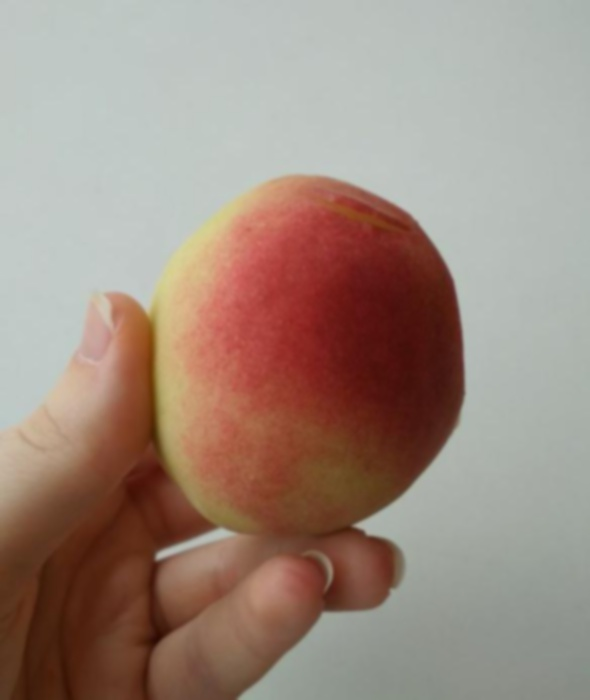
\includegraphics[width=0.3\textwidth]{peachs/blur}
	\end{center}
	\legend{Fonte Própria}
\end{figure} 

\item Nível-médio:
	São operações associadas a operações de segmentação de imagem ou reconhecimento de objetos na imagem \cite{marengoni:2009}. Um exemplo é ilustrado na \autoref{fig:segment}, onde foi feita a aplicação de um algoritmo de segmentação com base nas cores da imagem.
	
       \begin{figure}[ht]
	\caption{\label{fig:segment}Segmentação com base nas cores da imagem com sobreposição para identificação de pêssegos.}
	\begin{center}
	    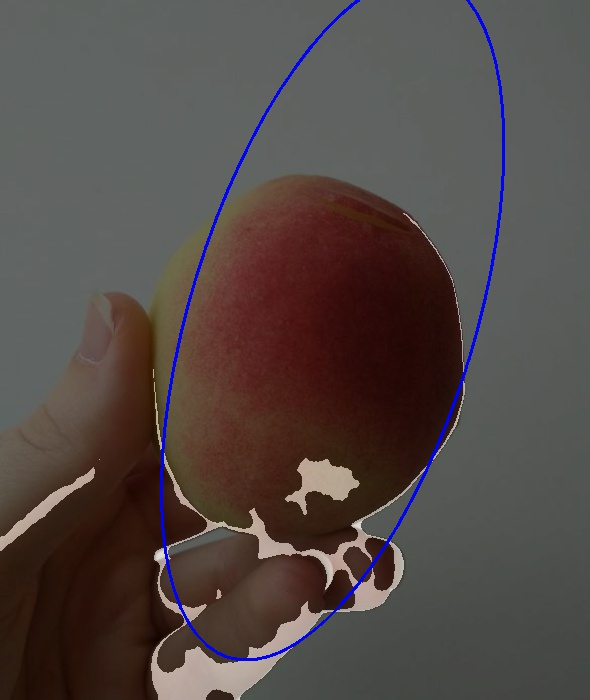
\includegraphics[width=0.3\textwidth]{peachs/identified}
	\end{center}
	\legend{Fonte Própria}
\end{figure}

\item Alto-nível:
São relacionados a tarefas de cognição associadas com a visão humana \cite{marengoni:2009}. Um exemplo pode ser visto na \autoref{fig:machineflow}, onde um \textit{framework} identificou a fruta com base em um modelo de dados, classificando e exibindo o resultado.
       \begin{figure}[ht]
	\caption{\label{fig:machineflow}Identificação de objetos utilizando aprendizado de máquina.}
	\begin{center}
	    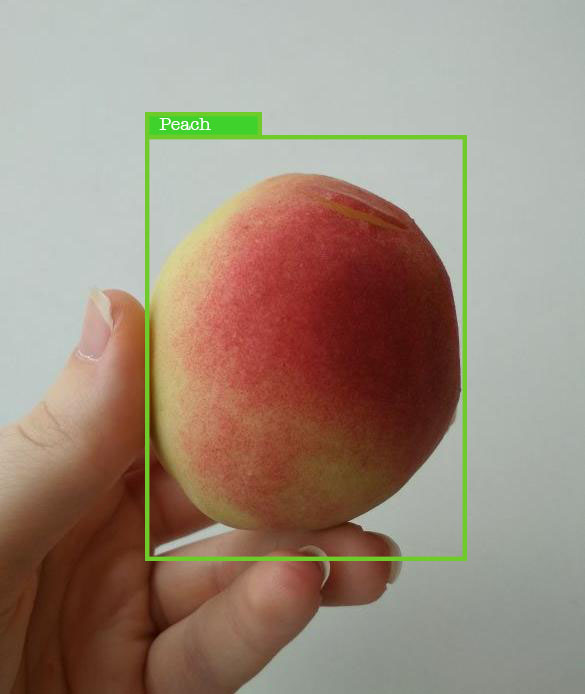
\includegraphics[width=0.3\textwidth]{peachs/tensorflow}
	\end{center}
	\legend{Fonte Própria}
\end{figure}
	
\end{itemize} 


% ----------------------------------------------
% ---------------------------------------------- 
\subsection{Representação de Imagens Digitais}
Uma imagem pode ser definida como uma função bidimensional, $f(x,y)$, onde $x$ e $y$ são coordenadas espaciais, e a amplitude de $f$ em qualquer par de coordenadas $(x,y)$ é chamada de intensidade da imagem, naquele determinado ponto. Quando $x,y$ e os valores de amplitude de $f$ são finitos, chamamos a imagem de imagem digital. Uma imagem digital é composta por um número finitos de elementos, cada um tendo seu próprio ponto e posição específicos. Esses elementos se referem à elementos de imagem, \textit{pels} e \textit{pixels} \cite{gonzalez1992digital}. 

O termo processamento de imagens digitais normalmente se referem ao processamento de imagens bidimensionais por computadores. Uma imagem digital é um vetor de números reais ou números complexos representados por uma quantidade finita de \textit{bits}.
Na representação de imagem devemos nos preocupar com a caracterização e quantidade de elementos que representam a imagem (\textit{pixels} ou \textit{pels}). Em geral qualquer função bidimensional que contém alguma informação pode ser considerada uma imagem. O principal requisito para o processamento de imagens digitais é que ela seja amostrada e logo em seguida quantificada. A taxa de amostragem, que são os \textit{pixels} por unidade de área, tem de ser grande o suficiente para preservar uma quantidade de informações úteis na imagem. A quantização da imagem é a conversão analógica para digital de uma imagem amostrada para um número finito de níveis de cinza \cite{jain1989fundamentals}.

 %\begin{figure}[h]
%	\caption{\label{fig:digitalproc}Típica sequência de processamento de imagem digital.}
%	\begin{center}
%	    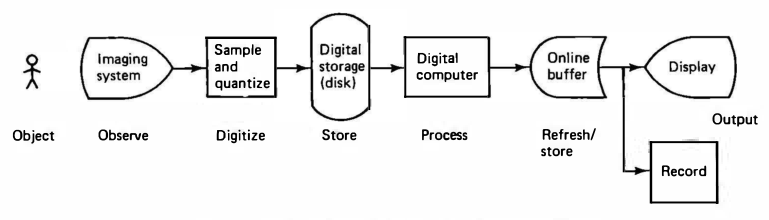
\includegraphics[width=.9\textwidth]{resources/digitalproc}
%	\end{center}
%	\legend{Fonte: \cite{jain1989fundamentals}}
%\end{figure}
Na \autoref{fig:matriz} é possível ver a convenção de coordenadas utilizada para representar imagens digitais segundo \citeonline{gonzalez1992digital}. O resultado da amostragem e quantização é uma matriz de números reais. Assumindo que a imagem $f(x,y)$ é amostrada, resultando uma imagem digital que possui $M$ linhas e $N$ colunas.


\begin{figure}[h]
	\caption{\label{fig:matriz}Amostragem de imagem e quantização}
	\begin{center}
	    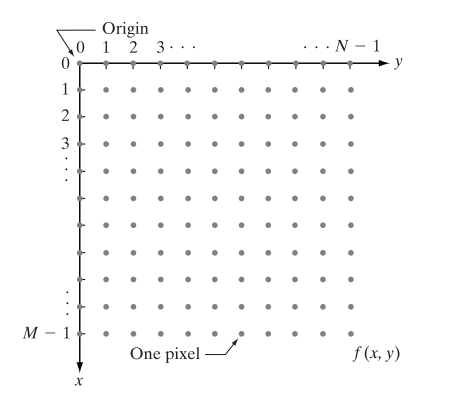
\includegraphics[width=.9\textwidth]{resources/matriz}
	\end{center}
	\legend{Fonte: \cite{gonzalez1992digital}}
\end{figure}


%\subsection{Pré-processamento de Imagem}

%\subsection{Segmentação e Detecção de Objetos}

%\subsection{Pós-Processamento}

\section{\textit{Frameworks} para identificação de imagem}

Nesta sessão iremos abordar \textit{frameworks} para identificação e classificação de imagens, onde são usando, as vantagens e desvantagens em  relação a métodos convencionais e tecnologias que utilizam \textit{frameworks} para suas atividades. %melhorar depois%

% \todo{falar sobre aprendizado de máquina na sua utilização no projeto: como caixa preta}
%De acordo com \cite{papag} As dificuldades na identificação de objetos de interesse do mundo real, como rostos e pessoas são dadas pela complexidade desses tipos de objetos, uma quantidade significante de variedade de cores e texturas e o contraste com o fundo da imagem. Em comparação com a classificação de padrões, onde é necessário decidir entre classes bem definidas, na detecção de objetos é necessário diferenciar a classe de objeto para o que é o resto. 

\subsection{\textit{Tensorflow}: Um \textit{Framework} de Código Aberto para Aprendizagem de Máquina}

Tensorflow é um \textit{framework} para operações computacionais, tendo uma grande biblioteca permitindo o desenvolvimento para diferentes plataformas, de \textit{clusters} de servidores até dispositivos móveis. Tensorflow tem grande facilidade de lidar com problemas de aprendizado de máquina e \textit{deep learning}, podendo ser usado em diversos domínios científicos \cite{tensorflow2015}. A utilização do \textit{framework} será de extrema importância nas classificações de imagens que serão processadas.

O campo de aprendizagem de máquina teve grandes progressos nos últimos anos, conseguindo alcançar níveis de abstração de imagem que alcançam a percepção humana. Um tipo de modelo que tem conseguido bons resultados, alcançando e até mesmo ultrapassando a capacidade humana em tarefas de reconhecimento de imagem são as \textbf{redes neurais convolutivas} (\textit{Convonlutional neural network}) \cite{Tensorflow2018}. Redes convolutivas estão no centro da maioria das soluções para problemas de reconhecimento de imagem \cite{SzegedyVISW15}.

O modelo que será utilizado no desenvolvivento desse trabalho será o \textit{Inception}, que segundo \citeonline{SzegedyVISW15} tem custo computacional bem menor que outros modelos, tornando a sua utilização viável para cenários com recursos limitados como em processamento móvel.

%============= PODEMOS DEIXAR O YOLO PRO TCC???? =================


%\subsection{YOLO: Detecção de Objetos em Tempo Real}
%\todo{fazer a mesma coisa pro YOLO (mesma coisa do tensorflow)}

%\todo[inline]{Ampliar a descrição e adição de exemplos}

%\section{Aprendizagem de máquina}
%Falar o que é. onde é usado, mostrar exemplos (muitas imagens), visão geral pra ter uma ideia do que é capaz

%\subsection{Redes Neurais}
%\todo{num sei}

%\subsection{Redes Neurais Convolutivas}
%\todo{num sei}

%\section{Reconhecimento de Padrões}


%\subsection{Aprendizado de máquina} 


%\subsection{Classificação de Padrões}


 
% \subsubsection{Homomorphic filtering} 
% 	O filtro homomórfico (\textit{homomorphic filter}) é um filtro de frequência usado para corrigir iluminações não uniformes e realçar o contraste na imagem processada \cite{bazeille2006}.
     
%  \begin{figure}[H]
% 	\centering
%     	\caption{\label{fig:homofilter}Homomorphic Filtering}
% 		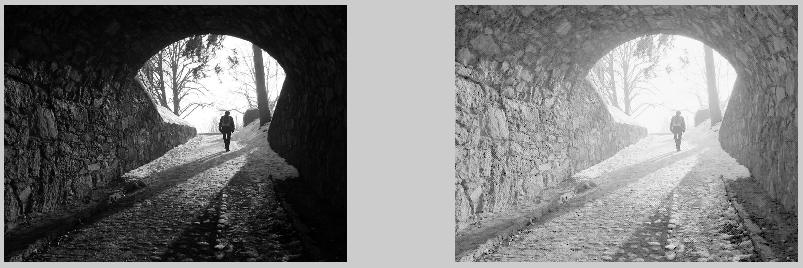
\includegraphics[width = 0.9\textwidth]	{resources/homofilter}
%     	\legend{\textit{Homomorphic filtering}, usando \textit{Butterworth High Pass Filter} para fazer a filtragem \cite{mathworks:2008}}.
% \end{figure}

%     %Considerando o modelo de reflectância, assumimos que uma imagem é o produto descrito pela equação:
%     \[
%     %	f (x,y) = i(x,y).r(x,y)
%     \]
%     %Sendo $f(x,y)$ é a imagem captada por um sensor ótico, $i(x,y)$ o fator multiplicativo de iluminação e $r(x,y)$ a função de reflectância. 
    

% \subsubsection{Anisotropic filtering}
% O Filtro anisotrópico permite a simplificação de atributos da imagem para melhorar a segmentação,  suavizando as partes homogêneas preservando as bordas e melhorando-as.

%  \begin{figure}[H]
% 	\centering
%     	\caption{\label{fig:anisifilter}Anisotropic Filtering}
% 		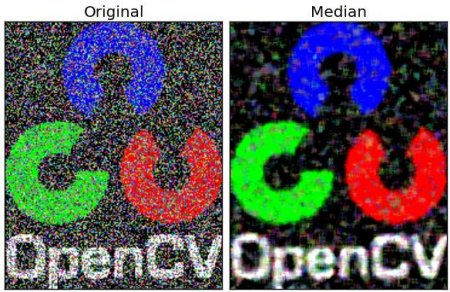
\includegraphics[width = 0.6\textwidth]	{resources/anisifilter}
%     	\legend{Fonte:\cite{mathworks:2008}}.
% % \end{figure}

% \subsection{Sensores de Aquisição de Imagens}
% Segundo \citeonline{Lu:2017}, o som pode ser usado para mapear ambientes, emitindo um pulso que reflete no fundo do oceano criando um sonograma. As imagens obtidas por este sonar se assemelham a imagens óticas, com níveis de detalhes bem superiores. O reflexo criado por esse sonar tem formato de leque, com a medida que o pulso se movimenta, os reflexos irão criar séries de linhas de imagem, perpendiculares ao feixe.  

% \subsection{Ferramentas para reconhecimento de images}
% \todo{Definir junto ao método proposto}


    
